\documentclass[a4paper,10pt]{article}
\usepackage[utf8]{inputenc}
\usepackage[T1]{fontenc}
\usepackage{lmodern}
\usepackage{graphicx}
\usepackage{tikz}
\usepackage{float}
\usepackage{longtable}
\usepackage{hyperref}
\begin{document}
\begin{titlepage}

\newcommand{\HRule}{\rule{\linewidth}{0.5mm}} % Defines a new command for the horizontal lines, change thickness here

\center % Center everything on the page
 
%----------------------------------------------------------------------------------------
%	HEADING SECTIONS
%----------------------------------------------------------------------------------------

\textsc{\LARGE Université de Mons}\\[1.5cm] % Name of your university/college
\textsc{\Large Compilation }\\[0.5cm] % Major heading such as course name

%----------------------------------------------------------------------------------------
%	TITLE SECTION
%----------------------------------------------------------------------------------------

\HRule \\[0.4cm]
{ \huge \bfseries Implémentation d'un moteur de template}\\[0.4cm] % Title of your document
\HRule \\[1.5cm]
 
%----------------------------------------------------------------------------------------
%	AUTHOR SECTION
%----------------------------------------------------------------------------------------

\begin{minipage}{0.4\textwidth}
\begin{flushleft} \large
\emph{Auteurs :}\\
Florent Delgrange \\
Clément Tamines
\end{flushleft}
\end{minipage}
~
\begin{minipage}{0.4\textwidth}
\begin{flushright} \large
\emph{Professeur:} \\
Véronique Bruyère
\emph{Assistant:} \\
Noémie Meunier
\end{flushright}
\end{minipage}\\[4cm]

% If you don't want a supervisor, uncomment the two lines below and remove the section above
%\Large \emph{Author:}\\
%John \textsc{Smith}\\[3cm] % Your name

%----------------------------------------------------------------------------------------
%	DATE SECTION
%----------------------------------------------------------------------------------------

{\large 23 mai 2016}\\[3cm] % Date, change the \today to a set date if you want to be precise

%----------------------------------------------------------------------------------------
%	LOGO SECTION
%----------------------------------------------------------------------------------------

%\includegraphics{Logo}\\[1cm] % Include a department/university logo - this will require the graphicx package
 
%----------------------------------------------------------------------------------------

\vfill % Fill the rest of the page with whitespace

\end{titlepage}

\newpage
\tableofcontents
\newpage

\section{Introduction}

Le but de ce projet est d'implémenter un moteur de template via la création d'un interpréteur du langage \textrm{Dumbo}. Ce moteur de template sera capable d'initialiser les 
variables contenues dans un fichier \textrm{data.dumbo}, il évaluera ensuite du code Dumbo injecté dans un fichier \textrm{template.dumbo} contenant du code et du texte. Un fichier
html sera alors produit, celui-ci contiendra le texte et le résultat de l'évaluation du code Dumbo. Il nous est demandé d'adapter la grammaire fournie dans l'énoncé pour 
qu'elle gère les expressions arithmétiques, les expressions booléennes ainsi que les structures de contrôle \textrm{if} et les boucles \textrm{for}.
Ce rapport a pout but d'expliquer les techniques que nous avons utilisées afin de réaliser cet interpréteur.

\section{Grammaire}
Afin d'ajouter les fonctionnalités demandées, nous avons ajouté certaines règles à la grammaire fournie dans l'énoncé.\newline La grammaire finale utilisée est la suivante : \\ \\
{\small
< programme > $\rightarrow$ < txt > | < txt > < programme >\\
< programme > $\rightarrow$ < dumbo\_bloc > \\
< programme > $\rightarrow$ < dumbo\_bloc > < programme > \\
< txt > $\rightarrow$ [a-zA-Z0-9; \& <> " - .\textbackslash / \textbackslash n \textbackslash p :, ]+ \\
< dumbo\_bloc > $\rightarrow$ {{ < expressions\_list > }} \\
< expressions\_list > $\rightarrow$ < expression > ; < expressions\_list >\\
< expressions\_list > $\rightarrow$ < expression > ; \\
< expression > $\rightarrow$ print < string\_expression > \\
< expression > $\rightarrow$ for < variable > in < string\_list > do < expressions\_list > endfor \\
< expression > $\rightarrow$ for < variable > in < variable > do < expressions\_list > endfor \\
< expression > $\rightarrow$ if < boolean\_expression > do < expression\_list > endif\\
< expression > $\rightarrow$ < variable > := < string\_expression > \\
< expression > $\rightarrow$ < variable > := < string\_list > \\
< expression > $\rightarrow$ < variable > := < operation > \\
< operation > $\rightarrow$ < integer > \\
< operation > $\rightarrow$ < variable > \\
< operation > $\rightarrow$ < operation > + < operation >\\
< operation > $\rightarrow$ < operation > - < operation >\\
< operation > $\rightarrow$ < operation > * < operation >\\
< operation > $\rightarrow$ < operation > / < operation >\\
< string\_expression > $\rightarrow$ < string > \\
< string\_expression > $\rightarrow$ < variable > \\
< string\_expression > $\rightarrow$ < string\_expression > . < string\_expression > \\
< string\_list > $\rightarrow$ ( < string\_list\_interior > ) \\
< string\_list\_interior > $\rightarrow$ < string >\\
< string\_list\_interior > $\rightarrow$ < string >, < string\_list\_interior > \\
< boolean\_expression > $\rightarrow$ < boolean > \\
< boolean\_expression > $\rightarrow$ < boolean\_expression > and < boolean\_expression > \\
< boolean\_expression > $\rightarrow$ < boolean\_expression > or < boolean\_expression > \\
< boolean\_expression > $\rightarrow$ < variable > < < variable >\\
< boolean\_expression > $\rightarrow$ < variable > > < variable >\\
< boolean\_expression > $\rightarrow$ < variable > = < variable >\\
< boolean\_expression > $\rightarrow$ < variable > != < variable >\\
< boolean > $\rightarrow$ [true|false]\\
< integer > $\rightarrow$ \textbackslash d+\\
< variable > $\rightarrow$ [a-z|A-Z]+[a-z|A-Z|0-9\_]*\\
< string > $\rightarrow$ '[a-zA-Z0-9; \& <> " - .\textbackslash / \textbackslash n\textbackslash p :, =]+' \\
}

Nous avons tout d'abord ajouté les règles < operation > qui permettent de stocker des entiers dans des variables : celles-ci peuvent donc contenir des entiers ou bien le résultat
de calculs sur des entiers. \newline Nous avons ensuite ajouté les expressions booléennes. Celles-ci sont utilisées comme condition dans 
le \textrm{if}.
Une expression booléenne peut être \textrm{true} ou \textrm{false} et peut aussi être le résultat d'une comparaison de deux entiers contenus dans des variables. Nous permettons d'effectuer des tests \textrm{or} et \textrm{and} entre plusieurs expressions booléennes.
\\ \\
Cette grammaire ainsi modifiée ne nous permet cependant pas certaines fonctionnalités, qui n'étaient pas expressément demandées dans l'énoncé :
\begin{itemize}
 \item Nous ne permettons pas de stocker des valeurs booléennes dans des variables, ces expressions étant seulement utilisées par la structure de contrôle \textrm{if}. 
 \item Nous ne permettons pas les comparaisons entre entiers et variables ou entre entiers. Lors des comparaisons, seules des entiers contenus dans des variables
 peuvent être utilisés.
\end{itemize}


\section{Arbre de dérivation}
Lors de l'analyse syntaxique, un arbre de dérivation est créé. Une fois une règle de la grammaire détectée, un noeud spécial correspondant à cette règle est
créé. Chaque nœud peut posséder ou non des fils et chaque type de nœud a un comportement différent lorsqu'il est exécuté. A la fin de l'analyse syntaxique,
la racine de l'arbre ainsi créé est retournée. Pour évaluer le code contenu dans l'arbre il ne nous reste plus qu'à demander l'exécution de sa racine, 
ce qui se fait en appelant la méthode \textrm{ex()} sur celle-ci. Cette méthode va être appellée récursivement par chaque nœud sur ses fils. La valeur retournée
par cette exécution d'un noeud correspond à l'évaluation de la partie du code dont ce nœud s'occupe. Lorsque tout les noeuds de l'arbre ont été exécutés, la racine 
renvoie une chaine de caractères correspondant à l'évaluation du code contenu dans l'arbre. Nous avons illustré ce principe via l'exemple de programme suivant : \\
\begin{verbatim}
<html>
{{
    print 'mot1'.'mot2';
}}
</html>
\end{verbatim}

Lorsque nous appliquerons notre analyseur syntaxique sur ce code, l'arbre suivant sera produit (cet arbre est une version simplifiée) :
\\
\begin{center}
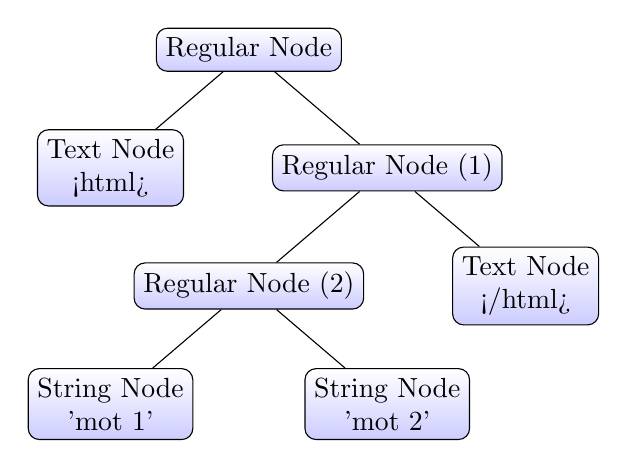
\begin{tikzpicture}[sibling distance=10em,
  every node/.style = {shape=rectangle, rounded corners,
    draw, align=center,
    top color=white, bottom color=blue!20}]]
    \node {Regular Node}
    child { node  {Text Node \\ <html>} }
    child{ node {Regular Node (1)}
        child { node {Regular Node (2)}
            child { node{String Node \\ 'mot 1'} }
            child { node{String Node \\ 'mot 2'} }
        }
        child { node{Text Node \\ </html>} }
    };
\end{tikzpicture}
\end{center}

\noindent
L'exécution de la racine via la méthode \textrm{ex()} aura le comportement suivant : \newline
\newline
La racine va demander le résultat de l'exécution de son fils gauche. Celui-ci étant un nœud texte, il va renvoyer le texte qu'il contient. \newline
La racine demande alors le résultat de l'exécution de son fils droit. Celui-ci étant aussi un nœud normal \texttt{(1)}, il va demander le résultat de l'exécution de son fils gauche.
Ce fils gauche \texttt{(2)} va lui aussi demander le résultat de son propre fils gauche. Ce nœud étant un noeud gérant les chaines de caractère, il va simplement renvoyer la chaine qu'il
contient en lui enlevant ses \texttt{'}. Il en va de même pour son fils droit. Le nœud normal \texttt{(2)} renvoie alors les deux chaines concaténées \texttt{mot1mot2}.
\newline
Le noeud \texttt{(1)} va demander le résultat de l'exécution de son fils droit. Celui-ci étant un nœud texte, il renverra le texte qu'il contient. Le nœud \texttt{(1)} termine alors son
exécution et renvoie \texttt{mot1mot2</html>}.\newline \newline
La racine possède alors le résultat de l'exécution de ses fils et renvoie la concaténation du résultat de leur exécution, qui correspond à l'évaluation du code contenu dans l'arbre. Ce résultat sera \texttt{<html>mot1mot2</html>}
\\
\\
En résumé, chaque nœud de l'arbre a une fonction spécifique et renverra le résultat de son exécution sous forme d'une chaine de caractère.\newline
Certains nœuds ont une fonction particulière qui ne renvoie aucune donnée. C'est le cas des nœuds d'assignation qui servent juste à ajouter une valeur dans le dictionnaire qui sert de 
table de variables (chaque variable étant une paire clé-valeur). Ce nœud, lorsqu'il est exécuté, se contente d'ajouter dans la table la clé qu'il contient et d'y associer la valeur demandée
par l'assignation (cette valeur résulte de l'exécution d'un autre nœud, par exemple d'un nœud réalisant des opérations arithmétiques). \\
Ajouter une règle à la grammaire sera alors facile puisqu'il suffira de créer un nœud qui gèrera le comportement voulu lors de la détection de cette règle. 

\section{Gestion du \textbf{if} et \textbf{for}}
Pour implémenter la structure de contrôle \textrm{if}, nous avons tout d'abord ajoutés les lexèmes \textbf{if} et \textbf{endif} dans l'analyseur lexical. Nous avons ensuite ajouté la 
règle suivante à la grammaire : < expression > $\rightarrow$ if < boolean\_expression > do < expression\_list > endif. \\
Lorsque cette règle est détectée par l'interpréteur, un nœud gérant le if est créé. Il possède une référence au nœud contenant la condition booléenne et une référence au nœud qui correspond
à l'action à effectuer si cette condition est vérifiée. Lors de l'exécution du nœud \textrm{if}, nous exécutons le nœud qui contient la condition booléenne. Le résultat de cette exécution
est récupéré et si la condition était vérifiée (\textrm{True} est renvoyé par le nœud) alors nous exécutons le nœud contenant l'action à effectuer et le résultat de cette exécution est renvoyé. \\
Au final, à la fin de l'exécution du nœud if, une chaine de caractère est renvoyée et celle-ci contient soit le résultat de l'exécution de l'action du if si la condition était vraie, soit une
chaine de caractères vide si la condition était fausse. 
\newline \newline
Le nœud gérant le \textrm{if} est implémenté de la manière suivante : 
\begin{verbatim}

class IfNode():
   def __init__(self, *args):
      # Le nœud prend en paramètre les nœuds contenant la condition 
      # et l'action du if, dans l'ordre fourni par la règle
      self.sons = args
         
   def ex(self):
      condition = self.sons[0]
      action = self.sons[1]

      # Le résultat est une chaine vide, sauf si la condition est vraie
      res = ""
      if(condition.ex()):
         # Si l'exécution du nœud contenant la condition est vraie, 
         # nous exécutons le nœud contenant l'action
         res += str(action.ex())
      return res
 
\end{verbatim}

Le \textrm{for} est géré avec la même logique que le \textrm{if}. Une fois une règle pour le \textrm{for} détectée, un nœud spécial est créé. Celui-ci prend en paramètre le nœud contenant
la variable, le nœud contenant la liste et le nœud contenant l'action à effectuer. \newline \newline Nous commençons d'abord par vérifier que la variable utilisée dans le for n'existe pas déjà dans la 
table des symboles. Si elle existe déjà, nous retenons sa valeur initiale pour la réassigner à la fin de la boucle. Nous récupérons ensuite la liste d'éléments contenue dans un nœud de variable
ou dans un nœud de liste via son exécution. Nous remarquons ici l'utilité d'avoir des nœuds différents implémentant chacun leur propre manière de s'exécuter. Si une variable contenant
une liste a été fournie, l'exécution du nœud contenant cette variable renverra la valeur associée au nom de la variable dans la table de variables. Si une liste a été directement fournie,
l'exécution du nœud renverra simplement cette liste. Cette méthode nous permet de ne pas faire la différence entre une liste contenue dans une variable ou une liste donnée directement. L'exécution
du nœud renverra une liste indépendamment de son type (si l'utilisateur respecte les conventions du language). Il nous suffit ensuite de parcourir chaque élément de la liste, d'assigner à la variable
la valeur de l'élément courant et d'effectuer l'action via l'exécution du nœud la contenant. Le résultat de cette exécution est récupéré dans une chaine de caractères et sera renvoyé une fois la boucle 
terminée. Il ne nous reste enfin qu'à rendre à la variable sa valeur initiale si elle en avait une et de renvoyer le résultat de l'exécution de la boucle.
\begin{verbatim}
 class ForNode():
   def __init__(self, *args):
      self.sons = args
         
   def ex(self):
      var_name = str(self.sons[0]) # Nom de la variable

      initial_value = "" # Valeur initiale de la variable

      # Si la variable existe déjà et a une valeur, nous la retenons
      if var_name in variables:
         initial_value = variables[var_name]

      # Récupérons la liste
      list_or_var = self.sons[1].ex()
      
      # Récupérons le nœud qui gère l'action
      action = self.sons[2]
      res = ""
      for var in list_or_var:
         variables[var_name] = var
         res+=action.ex()

      #Si la variable avait une valeur initiale, nous la réinstallons
      if initial_value != "":
         variables[var_name] = initial_value

      return res
\end{verbatim}

\section{Difficultés rencontrées}

Lors de nos tests, nous nous sommes rendus compte que l'analyseur lexical détectait mal certains lexèmes. Tout d'abord, le lexème texte était parfois détecté comme un lexème de variable
et vice-versa. La solution que nous avons trouvée a été de créer deux états dans l'analyseur lexical : l'un pour détecter des lexèmes lorsque nous étions hors d'un dumbo bloc 
contenant du code Dumbo et l'autre lorsque nous étions dans un dumbo bloc. Nous avons appelé cet état inBlock. Hors de cet état, seul le lexème texte peut être détecté. 
Lorsque le lexème HOOK\_OPEN signifiant l'entrée dans un dumbo bloc est rencontré, l'analyseur lexical entre dans l'état inBlock et seul les mots clés ainsi que les variables, entiers et 
chaines de caractères peuvent être détectés. L'analyseur ne pourra pas confondre les lexèmes texte et variables car chacun de ces lexèmes appartient à un état différent et l'analyseur 
ne peut détecter qu'un seul de ces lexèmes selon l'état dans lequel il se trouve. \\ \\
L'autre problème que nous avons rencontré est le suivant : dans l'état inBlock nous avons remarqué que les symboles réservés du langage ainsi que les nombres entiers 
étaient détectés comme des noms de variables dans certains cas. En effet le lexème variable étant le premier décrit dans cet état, lorsque l'analyseur rencontrait un \textrm{if} celui-ci 
était détecté comme une variable et rendait l'exécution impossible. Il en est de même pour \textrm{or}, \textrm{and}, ect. Nous avons réglé ce problème via l'utilisation d'un dictionnaire
de mots réservés dans le langage. Lorsque \textrm{if} est détecté comme une variable, ce dictionnaire est consulté avec \textrm{if} comme clé. Si if faisait partie du dictionnaire 
alors nous savons que c'est un mot réservé, la valeur correspondant à \textrm{if} dans le dictionnaire est le type correct de lexème à associer à \textrm{if}. Ceci n'empêche pas la détection
de mots réservés comme lexèmes de type variable mais permet la correction du type lorsque cette mauvaise détection arrive.\\ \\
En ce qui concerne les nombres entiers, nous avons empêché les noms de variable de commencer par un entier. Ceci empêche les entiers d'être confondus avec des noms de variable. 
Cette restriction ne nous a pas paru mauvaise car elle se fait dans de nombreux autres langages de programmation.

\end{document}
